\documentclass[a4paper]{article}
\usepackage{vntex}
\usepackage{a4wide,amssymb,epsfig,latexsym,array,hhline,fancyhdr}
\usepackage{amsmath}
\usepackage{amsthm}
\usepackage{multicol,longtable,amscd}
\usepackage{diagbox}%Make diagonal lines in tables
\usepackage{booktabs}
\usepackage{alltt}
\usepackage[framemethod=tikz]{mdframed}% For highlighting paragraph backgrounds
\usepackage{caption,subcaption}

\usepackage{lastpage}
\usepackage[lined,boxed,commentsnumbered]{algorithm2e}
\usepackage{enumerate}
\usepackage{color}
\usepackage{graphicx}							% Standard graphics package
\usepackage{array}
\usepackage{tabularx, caption}
\usepackage{multirow}
\usepackage{multicol}
\usepackage{enumitem}
\usepackage{rotating}
\usepackage{graphics}
\usepackage{geometry}
\usepackage{setspace}
\usepackage{epsfig}
\usepackage{tikz}
\usepackage{float}
\usetikzlibrary{arrows,snakes,backgrounds}
\usepackage[unicode]{hyperref}
\hypersetup{urlcolor=blue,linkcolor=black,citecolor=black,colorlinks=true} 
%\usepackage{pstcol} 								% PSTricks with the standard color package

%\usepackage{fancyhdr}
\setlength{\headheight}{40pt}
\pagestyle{fancy}
\fancyhead{} % clear all header fields
\fancyhead[L]{
 \begin{tabular}{rl}
    \begin{picture}(25,15)(0,0)
    \put(0,-8){
\includegraphics[width=8mm, height=8mm]{Image/hcmut.png}}
    %\put(0,-8){\epsfig{width=10mm,figure=hcmut.eps}}
   \end{picture}&
	%
\includegraphics[width=8mm, height=8mm]{hcmut.png} & %
	\begin{tabular}{l}
		\textbf{\bf \ttfamily Trường Đại Học Bách Khoa Tp.Hồ Chí Minh}\\
		\textbf{\bf \ttfamily Khoa Khoa Học và Kỹ Thuật Máy Tính}
	\end{tabular} 	
 \end{tabular}
}
\fancyhead[R]{
	\begin{tabular}{l}
		\tiny \bf \\
		\tiny \bf 
	\end{tabular}  }
\fancyfoot{} % clear all footer fields
\fancyfoot[L]{\scriptsize \ttfamily Thực tập Công nghệ phần mềm - Nhóm 2 - Dịch vụ chia sẻ nhà }
\fancyfoot[R]{\scriptsize \ttfamily Trang {\thepage}/\pageref{LastPage}}
\renewcommand{\headrulewidth}{0.3pt}
\renewcommand{\footrulewidth}{0.3pt}


%%%
\setcounter{secnumdepth}{4}
\setcounter{tocdepth}{3}
\makeatletter
\newcounter {subsubsubsection}[subsubsection]
\renewcommand\thesubsubsubsection{\thesubsubsection .\@alph\c@subsubsubsection}
\newcommand\subsubsubsection{\@startsection{subsubsubsection}{4}{\z@}%
                                     {-3.25ex\@plus -1ex \@minus -.2ex}%
                                     {1.5ex \@plus .2ex}%
                                     {\normalfont\normalsize\bfseries}}
\newcommand*\l@subsubsubsection{\@dottedtocline{3}{10.0em}{4.1em}}
\newcommand*{\subsubsubsectionmark}[1]{}
\makeatother

%%\everymath{\color{blue}}%make in-line maths symbols blue to read/check easily

\sloppy
\captionsetup[figure]{labelfont={small,bf},textfont={small,it},belowskip=-1pt,aboveskip=-9pt}
%space remove between caption, figure, and text
\captionsetup[table]{labelfont={small,bf},textfont={small,it},belowskip=-1pt,aboveskip=7pt}
%space remove between caption, table, and text

%\floatplacement{figure}{H}%forced here float placement automatically for figures
%\floatplacement{table}{H}%forced here float placement automatically for table
%the following settings (11 lines) are to remove white space before or after the figures and tables
%\setcounter{topnumber}{2}
%\setcounter{bottomnumber}{2}
%\setcounter{totalnumber}{4}
%\renewcommand{\topfraction}{0.85}
%\renewcommand{\bottomfraction}{0.85}
%\renewcommand{\textfraction}{0.15}
%\renewcommand{\floatpagefraction}{0.8}
%\renewcommand{\textfraction}{0.1}
\setlength{\floatsep}{5pt plus 2pt minus 2pt}
\setlength{\textfloatsep}{5pt plus 2pt minus 2pt}
\setlength{\intextsep}{10pt plus 2pt minus 2pt}

\begin{document}

\begin{titlepage}
\begin{center}
ĐẠI HỌC QUỐC GIA THÀNH PHỐ HỒ CHÍ MINH \\
TRƯỜNG ĐẠI HỌC BÁCH KHOA \\
KHOA KHOA HỌC - KỸ THUẬT MÁY TÍNH 
\end{center}

\vspace{1cm}

\begin{figure}[h!]
\begin{center}

\includegraphics[width=3cm]{Image/hcmut.png}
\end{center}
\end{figure}

\vspace{0.5cm}

\begin{center}
\textbf{\huge HỆ THỐNG CHIA SẺ NHÀ}\\
\vspace{0.25cm}
\textbf{\Huge \textcolor{red}{Diamond Stay}}\\
\textbf{\huge \textcolor{blue}{Phiên bản: 1.11}}\\
\vspace{1.5cm}
\textcolor{red}{\textbf{\huge  Nhóm 2}}

\end{center}

\vspace{0.7cm}


\begin{table}[h]
\begin{tabular}{rrl}
\hspace{5 cm} & GVHD: & Trương Tuấn Anh\\
& SV: & Đinh Minh Tân - 1613074 \\
& & Văn Tiến Cường - 1610386\\
& & Nguyễn Phan Đăng Khoa - 1611626\\
& & Lê Đăng Bảo - 1610165\\
& & Trần Ngọc Tín - 1613575\\
\vspace{2.3cm}

\end{tabular}
\end{table}

\begin{center}
{\footnotesize Tp. Hồ Chí Minh, Tháng 4/2019}
\end{center}
\end{titlepage}

%Mục lục
\newpage
\thispagestyle{empty}
\tableofcontents

%Danh sách hình
\newpage
\thispagestyle{empty}
\listoffigures
\newpage 

\section{Lịch sử sửa đổi}
\begin{center}
		\begin{longtable}{ | c | c | p{5cm} |c|}
		\hline 
		\textbf{Ngày} & \textbf{Phiên bản} & \textbf{Thay đổi} & \textbf{Người thay đổi} \\ \hline 
		09/03/2019 & 1.0 & Giới thiệu, Mô tả tổng quan & Team \\ \hline 
		17/03/2019 & 1.1a & Thêm mô tả chi tiết các use case: Duyệt tin, Thêm khuyến mại hệ thống, Thêm khuyến mại riêng, Xóa khuyến mại hệ thống, Xóa khuyến mại riêng & Tân \\ \hline  
		
		17/03/2019 & 1.1b & Thêm mô tả chi tiết các use case: Tìm kiếm, lọc homestay; Chức năng đặt phòng homestay. & Khoa\\ \hline
		
		17/03/2019 & 1.1c & Thêm mô tả các module Theo dõi tình trạng đặt phòng (cho chủ nhà) và Tin nhắn (cho chủ nhà.) & Cường \\ \hline
		
		17/03/2019 & 1.1d & Thêm mô tả chi tiết các use case: Thêm tin mới, duyệt các tin đã đăng, ẩn tin đã đăng, chỉnh  sửa và gửi lại tin đã bị từ chối. & Bảo \\ \hline  
		
		17/03/2019 & 1.1f & Thêm mô tả chi tiết các use case: Bình luận cho nhà, rating cho nhà. & Tín \\ \hline
		
		19/03/2019 & 1.2 & Thêm đặc tả các yêu cầu phi chức năng & Tân \\ \hline 
		28/03/2019 & 1.3a &  Thêm usecase diagram cho 2 module: Duyệt tin, Quản lí khuyến mại & Tân \\ \hline 
		28/03/2019 & 1.3b &  Thêm usecase diagram cho 2 module: TIme kiếm và lọc; Đặt phòng & Khoa \\ \hline 
		30/03/2019 & 1.4a & Cập nhật mô tả chi tiết các use case: Duyệt tin, Thêm khuyến mại hệ thống, Thêm khuyến mại riêng, Xóa khuyến mại hệ thống, Xóa khuyến mại riêng & Tân \\ \hline 
		30/03/2019 & 1.4b & Thêm sequence diagram cho các usecase: Tìm kiếm, lọc và đặt phòng & Khoa \\ \hline 
		30/03/2019 & 1.4c & Cập nhật đặc tả các yêu cầu phi chức năng & Cường \\ \hline
		30/03/2019 & 1.4d & Cập nhật use-case, mô tả chi tiết về use-case, sequence diagram: Thêm mới, Xem danh sách tin. & Bảo \\ \hline
		
		30/03/2019 & 1.4e & Thêm use case và chi tiết các chức năng thuộc nhóm tin nhắn cho khách thuê. & Cường \\ \hline
		
		06/04/2019 & 1.5a & Thêm UI cho các giao diện: Thêm khuyến mãi, Quản lí tin đăng, Duyệt tin chỗ ở mới, Xóa khuyến mại & Tân \\ \hline 
		06/04/2019 & 1.5b & Thêm UI cho các giao diện: Thêm giao diện tìm kiếm; Lọc kết quả, đặt phòng và thanh toán yêu cầu đặt homestay & Khoa \\ \hline
		06/04/2019 & 1.5c & Thêm UI cho các chức năng: Đăng tin mới, xem danh sách tin, ẩn tin, chỉnh sửa tin bị trả lại. & Bảo \\ \hline
		06/04/2019 & 1.5d & Thêm UI cho các chức năng: xem danh sách phòng, xem danh sách tin nhắn, xem chi tiết tin nhắn, trả lời tin nhắn (dành cho chủ nhà). & Cường \\ \hline
		06/04/2019 & 1.5e & Thêm UI cho các chức năng: xem danh sách phòng, xem danh sách tin nhắn, xem chi tiết tin nhắn, trả lời tin nhắn (dành cho chủ nhà). & Cường \\ \hline
		06/04/2019 & 1.5f & Chỉnh sửa UI cho chức năng xếp hạng nhà & Tín \\ \hline
		12/04/2019 & 1.6 & Cập nhật sơ đồ use case tổng quát cho toàn hệ thống & Tân \\ \hline
		\end{longtable}
\end{center}

\newpage 

\section{Giới thiệu}
Ngày nay, kinh tế chia sẻ là một khái niệm không còn xa lạ với nhiều người.
Các mô hình kinh tế chia sẻ như chia sẻ xe, chia sẻ nhà,... ngày càng phổ biến.
Đối với chia sẻ xe thì ta có thể nhìn vào Grab, GoViet, ... là những ví dụ điển
hình nhất. Ý tưởng của chia sẻ xe đơn giản là việc khi người dân di chuyển thay
vì vị trí ghế ngồi sau bỏ trống, người ta có thể chia sẻ vị trí này với người khác
và thu một khoản phí thích hợp. Đối với chia sẻ nhà, việc áp dụng kinh tế chia
sẻ vào giúp các chủ nhà trọ, homestay có phòng trống cần cho thuê và các khách
du lịch, người dân cần có nhu cầu lưu trú trong ngắn hạn có thể kết nối nhanh
chóng và giao dịch dễ dàng hơn. Ở đây hệ thống đóng vai trò là bên trung gian
hỗ trợ giúp chủ nhà và người đi thuê và thu phí hoa hồng khi chủ nhà và người
đi thuê giao dịch thành công chứ thực chất hệ thống không bán hay kinh doanh
bất động sản gì cả. Trong môn học này nhóm quyết định xây dựng hệ thống
giúp hỗ trợ chia sẻ nhà.

\section{Tổng quan hệ thống}
Hệ thống Diamond Stay được chia thành các module sau:
\begin{itemize}
	\item \textbf{Module 1 \textcolor{red}{(Tân)}:} Duyệt thông tin về yêu cầu thêm chỗ ở mới từ chủ nhà (Dành cho quản lí hệ thống) 
	\item \textbf{Module 2 \textcolor{red}{(Tân)}:} Quản lí khuyến mại (Khuyến mại của chủ nhà và khuyến mại của hệ thống).
	\item \textbf{Module 3 \textcolor{red}{(Tín)}:} Bình luận và rating cho nhà.
	\item \textbf{Module 4 \textcolor{red}{(Bảo)}:} Yêu cầu tạo tin mới, quản lý các tin đã gửi 
	\item \textbf{Module 5 \textcolor{red}{(Khoa)}:} Tìm kiếm và lọc kết quả; Đặt phòng homestay 
	\item \textbf{Module 6 \textcolor{red}{(Cường)}:} Theo dõi tình trạng đặt phòng cho chủ nhà
	\item \textbf{Module 7 \textcolor{red}{(Cường)}:} Các chức năng về nhắn tin cho khách thuê
	\item \textbf{Module 8 \textcolor{red}{(Cường)}:} Các chức năng về nhắn tin cho chủ nhà 
\end{itemize}
\newpage 
\begin{figure}[H]
	\centering
	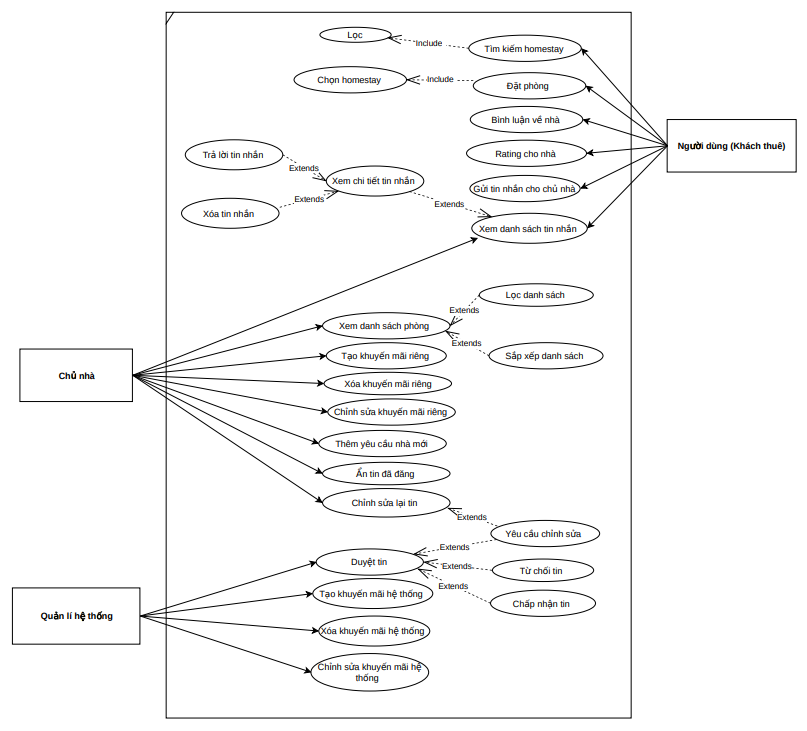
\includegraphics[width=17cm, height= 17cm]{Image/ucFull.png}
	\vspace{0.5cm}
	\caption{Lược đồ usecase của toàn hệ thống}
\end{figure}

\newpage 
%%%%%%% USE CASE %%%%%%%%%%%%%%%%

\subsection{Module 3: Bình luận và rating cho nhà}
\begin{figure}[!h]
	\centering
	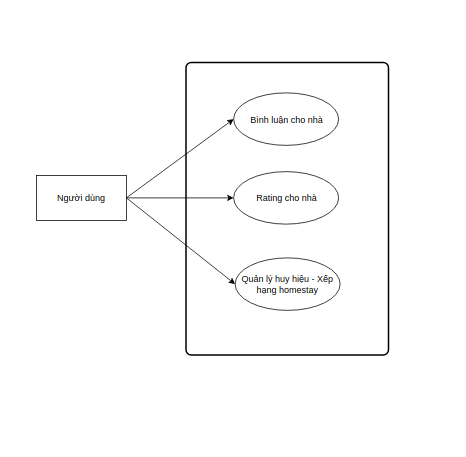
\includegraphics[width=10cm]{Image/tin-usecase.png}
	\caption{Lược đồ use case của Module 3: Bình luận và rating cho nhà}
\end{figure}
\subsubsection{User Story}
\textit{Diamond Stay} là một hệ thống trung gian giữa người cần thuê nhà và người cho thuê nhà. Hệ thống sẽ thu phí hoa hồng mỗi khi có lượt giao dịch thành công giữa chủ nhà và người cho thuê. Chủ nhà muốn thêm chỗ ở mới cần cho thuê thì cần gửi yêu cầu thêm chỗ ở mới lên hệ thống. Để thông tin về chỗ ở mới này xuất hiện trên trang web chính của \textit{Diamond Stay} để khách thuê nhà có thể thấy và đặt phòng thì tin đăng này cần phải được duyệt trước để đảm bảo tin đăng là hợp lệ, không phải là spam hay tin giả do một số đối tượng cố tình phá hoại hệ thống gửi lên. Những tin đăng loại này sẽ gây loãng hệ thống và gây khó khăn cho người dùng. Việc duyệt tin sẽ được những quản lí của hệ thống thực hiện. Hệ thống sẽ có một số tiêu chí để xác định tin đăng là hợp lệ hay không. Dựa vào đó quản lí có thể dựa vào để có thể quyết định trạng thái kế tiếp của 1 tin đăng. Các trạng thái này có thể là:
\begin{itemize}
	\item \textit{Thành công}: Tin đăng hợp lệ và được hiển thị lên trang web của Diamond Stay để khách thuê có thể nhìn thấy và đặt phòng 
	\item \textit{Bị từ chối}: Tin đăng không hợp lệ.
	\item \textit{Yêu cầu chỉnh sửa}: Tin đăng cần sửa đổi, bổ sung một số thông tin để hợp lệ. Chủ nhà sau khi sửa đổi và bổ sung có thể resubmit lại tin này.
\end{itemize}
Khi quản lí duyệt một tin là \textit{Bị từ chối} thì quản lí cần cung cấp lí do tin đăng bị từ chối, còn nếu tin đăng bị đánh giá là \textit{Yêu cầu chỉnh sửa} thì quản lí cần cung cấp chi tiết những nội dung nào cần chỉnh sửa, những nội dung nào chưa hợp lệ.
\subsubsection{Các usecase chi tiết}
\begin{figure}[!h]
	\centering
	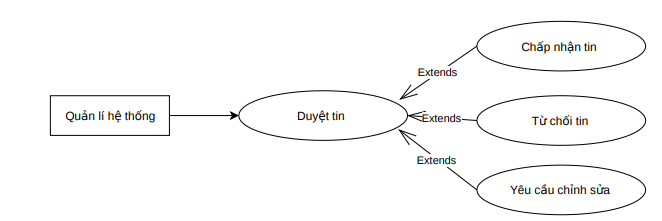
\includegraphics[width=12cm]{Image/module1.png}
	\vspace{0.5cm}
	\caption{Lược đồ use case của Module 1: Duyệt tin đăng yêu cầu thêm chỗ ở mới từ chủ nhà}
\end{figure}
\subsubsubsection{Use Case 1: Duyệt tin.}
\begin{figure}[!h]
	\centering
	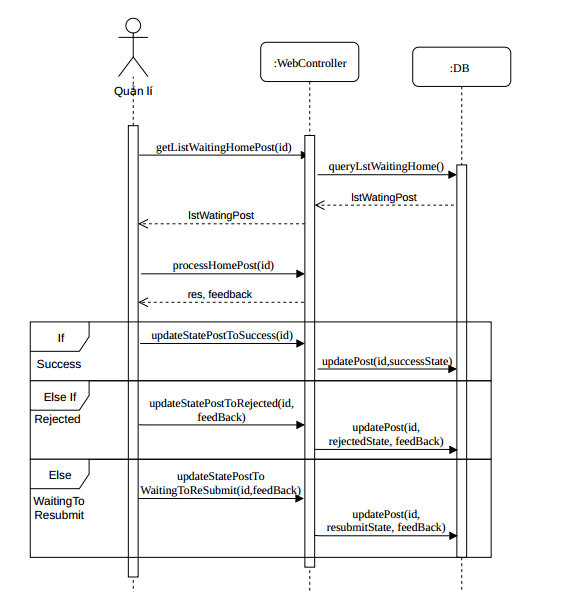
\includegraphics[width=13cm]{Image/duyetTinSequence.png}
	\caption{Sequence Diagram cho usecase Duyệt tin}
\end{figure}
\begin{center}
	\begin{longtable}{ | l |p{10cm}|}
		\hline
		\textbf{Tên usecase} & Duyệt tin \\ \hline
		\textbf{Người tương tác} & Quản lí hệ thống \\ \hline   
		\textbf{Mô tả} &  Cho phép người quản lí của hệ thống có thể duyệt qua các yêu cầu thêm nhà mới từ các chủ nhà. Việc duyệt tin để đảm bảo chất lượng của các bài đăng trên trang web của hệ thống.\\ \hline  
		\textbf{Người tạo:} \textit{Đinh Minh Tân} & \textbf{Cập nhật lần cuối bởi:} \textit{Đinh Minh Tân} \\ \hline
		\textbf{Ngày tạo:} \textit{22/03/2019} & \textbf{Lần cuối cập nhật:} \textit{30/03/2019} \\ \hline
		\textbf{Tiền điều kiện} &  Người dùng đã đăng nhập vào hệ thống bằng quyền của người quản lí, người dùng đang ở màn hình index của trang web. \\ \hline 
		\textbf{Hậu điều kiện} &  Quản lí quay về màn hình quản lí các tin chưa duyệt. \\ \hline 
		\textbf{Luồng cơ bản} & 
		\begin{enumerate}
			\item Quản lí nhấn tab Quản lí tin đăng.
			\item Hệ thống hiển thị 2 option cho quản lí bao gồm: Tin chưa duyệt, Tin đã duyệt.
			\item Quản lí chọn Tin chưa duyệt.
			\item Hệ thống hiển thị danh sách các tin chưa được duyệt, đang đợi duyệt.
			\item Người quản lí chọn một tin bất kì mà mình sẽ duyệt trong danh sách tin hiện ra.
			\item Hệ thống hiển thị tất cả thông tin của homestay cần được duyệt, trong đó có 3 option để duyệt: Chấp nhận, Từ chối và Yêu cầu chỉnh sửa.
			\item Quản lí sau khi duyệt tất cả các thông tin đầy đủ và hợp lệ, chọn option Chấp nhận và nhấn Button OK để xác nhận quyết định.
			\item Hệ thống hiện ra thông báo đã xác nhận thành công và tin đăng về homestay đã được đăng thành công lên trang web để khách thuê có thể thấy và đặt.
			\item Hệ thống quay về màn hình quản lí các tin chưa duyệt để quản lí có thể duyệt tin khác (nếu cần).
		\end{enumerate} \\ \hline 
		\textbf{Luồng thay thế} & 
		\begin{itemize} 
			\item \textit{Luồng thay thế 1}
			\begin{enumerate}
				\item Tại bước 4, hệ thống không tìm được tin nào chưa được duyệt thì sẽ in ra thông báo "Không có tin đăng nào cần duyệt" kết thúc chức năng này tại đây.
			\end{enumerate}
			
			\item \textit{Luồng thay thế 2}
			\begin{enumerate}
				\item Tại bước 6, quản lí chọn option Từ chối.
				\item Hệ thống hiện thị một form để quản lí điền lí do tin đăng bị từ chối. Sau khi hoàn thành xong form, quản lí nhấn OK.
				\item Hệ thống xác nhận tin đã bị từ chối và gửi kết quả về cho chủ nhà 
				\item Tiếp tục tại bước 9 của luồng cơ bản.
			\end{enumerate}
			
			\item \textit{Luồng thay thế 3}
			\begin{enumerate}
				\item Tại bước 6, quản lí chọn option Yêu cầu sửa đổi.
				\item Hệ thống hiện thị một form để quản lí điền những yêu cầu mà chủ nhà cần sửa đổi hoặc bổ sung thêm. Sau khi hoàn thành xong form, quản lí nhấn OK.
				\item Hệ thống đánh dấu chuyển tin sang dạng đợi và chuyển vào mục tin cần sửa đổi và resubmit lại bên phía chủ nhà.
				\item Tiếp tục tại bước 9 của luồng cơ bản.
			\end{enumerate}
		\end{itemize} \\ \hline 
		\textbf{Ngoại lệ}  & Không có \\
		\hline
	\end{longtable}
\end{center}
\subsubsection{Quản lý huy hiệu, xếp hạng các homestay}
\subsubsubsection{User Story}
\textit Từ kết quả rating,{Diamond Stay} sẽ quản lí huy hiệu và xếp hạng các homestay. Dựa trên cơ sở này, người dùng có thể dễ dàng biết được mức độ chuyên nghiệp cũng như chất lượng thực sự của homestay

\subsubsubsection{Mô tả các use case}
\begin{enumerate}[label=\textbf{(\alph*)}]
    \begin{figure}[!h]
        	\centering
        	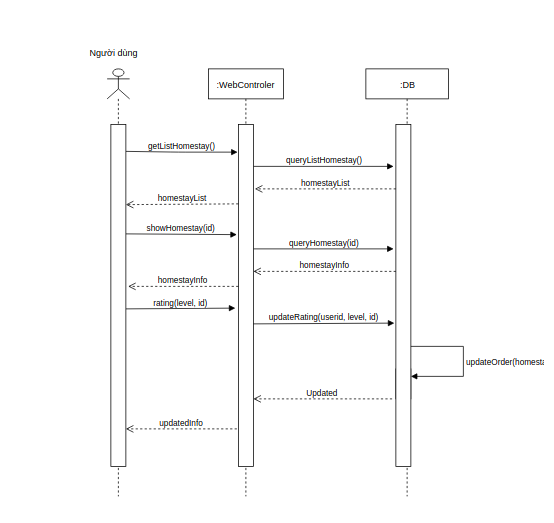
\includegraphics[width=13cm]{Image/tin-sequence-homstay-order.png}
        	\caption{Sequence Diagram cho usecase xếp hạng các homestay}
    \end{figure}
	\item \textbf{Usecase 3: Quản lý huy hiệu và xếp hạng các homestay.}
	\begin{center}
		\begin{longtable}{ | l |p{10cm}|}
			\hline
			\textbf{Tên usecase} & Quản lý huy hiệu và xếp hạng các homestay \\ \hline
			\textbf{Người tương tác} & Người dùng hệ thống \\ \hline   
			\textbf{Mô tả} &  Hệ thống tự động cập nhật huy hiệu và thứ hạng của nhà sau khi có 1 ratingmới của nhà xuất hiện. \\ \hline  
			\textbf{Người tạo:} \textit{Trần Ngọc Tín} & \textbf{Cập nhật lần cuối bởi:} \textit{Trần Ngọc Tín} \\ \hline
			\textbf{Ngày tạo:} \textit{22/03/2019} & \textbf{Lần cuối cập nhật:} \textit{30/03/2019} \\ \hline
			\textbf{Tiền điều kiện} &  Người dùng nào đó rating nhà. \\ \hline 
			\textbf{Hậu điều kiện} &  Thông tin về huy hiệu và thứ hạng của nhà đó được cập nhật \\ \hline 
			\textbf{Luồng cơ bản} & 
			\begin{enumerate}
		\item Người dùng rating nhà
		\item Hệ thống tính toán lại mức rating trung bình của nhà đó cũng như tổng số rating
		\item Hệ thống cập nhật lại huy hiệu cho nhà dựa theo mức rating trung bình và tổng số rating, chi tiết như sau:
		\begin{itemize}
		    \item Với nhà có tổng rating dưới 5: huy hiệu là "Nhà mới"
		    \item Với nhà đạt được tổng rating > 5 và <= 10: huy hiệu là "Nhà phổ biến"
		    \item Với nhà có tổng rating > 10, lúc này sẽ tính huy hiệu theo rating trung bình
		    \begin{itemize}
		        \item Với rating trung bình < 1: huy hiệu "Nhà quá tệ"
		        \item Với rating trung bình >= 1 và < 2: huy hiệu "Nhà tệ"
		        \item Với rating trung bình >= 2 và < 3: huy hiệu "Nhà tạm được"
		        \item Với rating trung bình >= 3 và < 4: huy hiệu "Nhà tốt"
		        \item Với rating trung bình >= 4 và <= 5: huy hiệu "Nhà tuyệt vời"
		    \end{itemize}
		\end{itemize}
		\item Hệ thống tính toán lại thứ tự ưu tiên của nhà theo mức rating trung bình mới, nhà nào có mức rating trung bình cao thì xếp hạng cao, nếu 2 nhà có mức rating trung bình bằng nhau thì dựa vào tổng số rating để xếp hạng, nhà nào có tổng rating cao hơn thì xếp hạng cao hơn
			\end{enumerate} \\ \hline
			\textbf{Luồng thay thế} & Không có \\ \hline
			\textbf{Ngoại lệ}  & Không có \\
			\hline
		\end{longtable}
	\end{center}
\end{enumerate}
\subsection{Module 3: Bình luận và rating cho nhà}
\begin{figure}[!h]
	\centering
	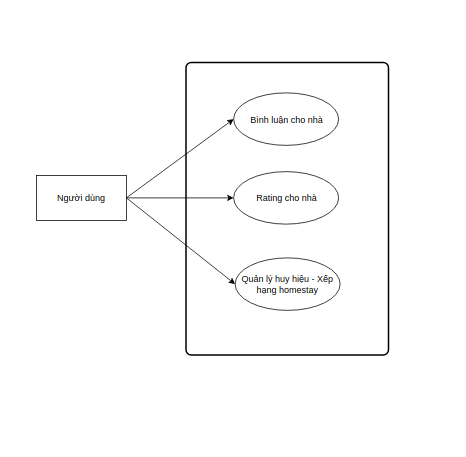
\includegraphics[width=10cm]{Image/tin-usecase.png}
	\caption{Lược đồ use case của Module 3: Bình luận và rating cho nhà}
\end{figure}
\subsubsection{User Story}
\textit{Diamond Stay} là một hệ thống trung gian giữa người cần thuê nhà và người cho thuê nhà. Hệ thống sẽ thu phí hoa hồng mỗi khi có lượt giao dịch thành công giữa chủ nhà và người cho thuê. Chủ nhà muốn thêm chỗ ở mới cần cho thuê thì cần gửi yêu cầu thêm chỗ ở mới lên hệ thống. Để thông tin về chỗ ở mới này xuất hiện trên trang web chính của \textit{Diamond Stay} để khách thuê nhà có thể thấy và đặt phòng thì tin đăng này cần phải được duyệt trước để đảm bảo tin đăng là hợp lệ, không phải là spam hay tin giả do một số đối tượng cố tình phá hoại hệ thống gửi lên. Những tin đăng loại này sẽ gây loãng hệ thống và gây khó khăn cho người dùng. Việc duyệt tin sẽ được những quản lí của hệ thống thực hiện. Hệ thống sẽ có một số tiêu chí để xác định tin đăng là hợp lệ hay không. Dựa vào đó quản lí có thể dựa vào để có thể quyết định trạng thái kế tiếp của 1 tin đăng. Các trạng thái này có thể là:
\begin{itemize}
	\item \textit{Thành công}: Tin đăng hợp lệ và được hiển thị lên trang web của Diamond Stay để khách thuê có thể nhìn thấy và đặt phòng 
	\item \textit{Bị từ chối}: Tin đăng không hợp lệ.
	\item \textit{Yêu cầu chỉnh sửa}: Tin đăng cần sửa đổi, bổ sung một số thông tin để hợp lệ. Chủ nhà sau khi sửa đổi và bổ sung có thể resubmit lại tin này.
\end{itemize}
Khi quản lí duyệt một tin là \textit{Bị từ chối} thì quản lí cần cung cấp lí do tin đăng bị từ chối, còn nếu tin đăng bị đánh giá là \textit{Yêu cầu chỉnh sửa} thì quản lí cần cung cấp chi tiết những nội dung nào cần chỉnh sửa, những nội dung nào chưa hợp lệ.
\subsubsection{Các usecase chi tiết}
\begin{figure}[!h]
	\centering
	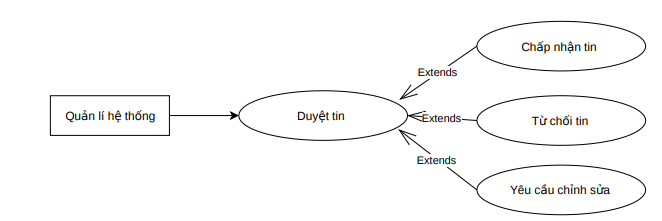
\includegraphics[width=12cm]{Image/module1.png}
	\vspace{0.5cm}
	\caption{Lược đồ use case của Module 1: Duyệt tin đăng yêu cầu thêm chỗ ở mới từ chủ nhà}
\end{figure}
\subsubsubsection{Use Case 1: Duyệt tin.}
\begin{figure}[!h]
	\centering
	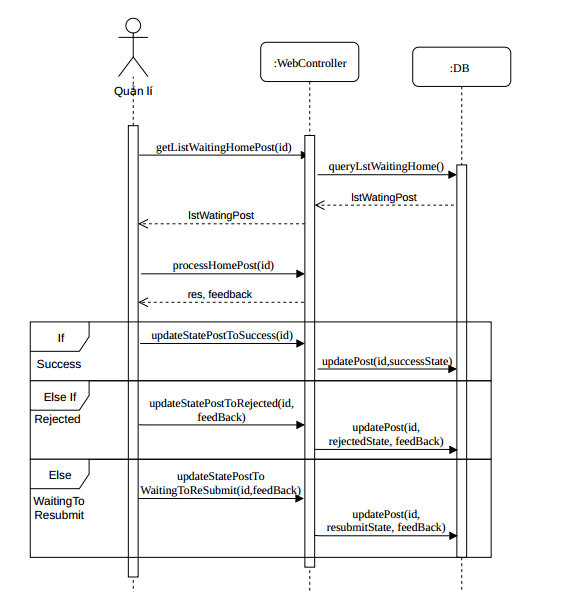
\includegraphics[width=13cm]{Image/duyetTinSequence.png}
	\caption{Sequence Diagram cho usecase Duyệt tin}
\end{figure}
\begin{center}
	\begin{longtable}{ | l |p{10cm}|}
		\hline
		\textbf{Tên usecase} & Duyệt tin \\ \hline
		\textbf{Người tương tác} & Quản lí hệ thống \\ \hline   
		\textbf{Mô tả} &  Cho phép người quản lí của hệ thống có thể duyệt qua các yêu cầu thêm nhà mới từ các chủ nhà. Việc duyệt tin để đảm bảo chất lượng của các bài đăng trên trang web của hệ thống.\\ \hline  
		\textbf{Người tạo:} \textit{Đinh Minh Tân} & \textbf{Cập nhật lần cuối bởi:} \textit{Đinh Minh Tân} \\ \hline
		\textbf{Ngày tạo:} \textit{22/03/2019} & \textbf{Lần cuối cập nhật:} \textit{30/03/2019} \\ \hline
		\textbf{Tiền điều kiện} &  Người dùng đã đăng nhập vào hệ thống bằng quyền của người quản lí, người dùng đang ở màn hình index của trang web. \\ \hline 
		\textbf{Hậu điều kiện} &  Quản lí quay về màn hình quản lí các tin chưa duyệt. \\ \hline 
		\textbf{Luồng cơ bản} & 
		\begin{enumerate}
			\item Quản lí nhấn tab Quản lí tin đăng.
			\item Hệ thống hiển thị 2 option cho quản lí bao gồm: Tin chưa duyệt, Tin đã duyệt.
			\item Quản lí chọn Tin chưa duyệt.
			\item Hệ thống hiển thị danh sách các tin chưa được duyệt, đang đợi duyệt.
			\item Người quản lí chọn một tin bất kì mà mình sẽ duyệt trong danh sách tin hiện ra.
			\item Hệ thống hiển thị tất cả thông tin của homestay cần được duyệt, trong đó có 3 option để duyệt: Chấp nhận, Từ chối và Yêu cầu chỉnh sửa.
			\item Quản lí sau khi duyệt tất cả các thông tin đầy đủ và hợp lệ, chọn option Chấp nhận và nhấn Button OK để xác nhận quyết định.
			\item Hệ thống hiện ra thông báo đã xác nhận thành công và tin đăng về homestay đã được đăng thành công lên trang web để khách thuê có thể thấy và đặt.
			\item Hệ thống quay về màn hình quản lí các tin chưa duyệt để quản lí có thể duyệt tin khác (nếu cần).
		\end{enumerate} \\ \hline 
		\textbf{Luồng thay thế} & 
		\begin{itemize} 
			\item \textit{Luồng thay thế 1}
			\begin{enumerate}
				\item Tại bước 4, hệ thống không tìm được tin nào chưa được duyệt thì sẽ in ra thông báo "Không có tin đăng nào cần duyệt" kết thúc chức năng này tại đây.
			\end{enumerate}
			
			\item \textit{Luồng thay thế 2}
			\begin{enumerate}
				\item Tại bước 6, quản lí chọn option Từ chối.
				\item Hệ thống hiện thị một form để quản lí điền lí do tin đăng bị từ chối. Sau khi hoàn thành xong form, quản lí nhấn OK.
				\item Hệ thống xác nhận tin đã bị từ chối và gửi kết quả về cho chủ nhà 
				\item Tiếp tục tại bước 9 của luồng cơ bản.
			\end{enumerate}
			
			\item \textit{Luồng thay thế 3}
			\begin{enumerate}
				\item Tại bước 6, quản lí chọn option Yêu cầu sửa đổi.
				\item Hệ thống hiện thị một form để quản lí điền những yêu cầu mà chủ nhà cần sửa đổi hoặc bổ sung thêm. Sau khi hoàn thành xong form, quản lí nhấn OK.
				\item Hệ thống đánh dấu chuyển tin sang dạng đợi và chuyển vào mục tin cần sửa đổi và resubmit lại bên phía chủ nhà.
				\item Tiếp tục tại bước 9 của luồng cơ bản.
			\end{enumerate}
		\end{itemize} \\ \hline 
		\textbf{Ngoại lệ}  & Không có \\
		\hline
	\end{longtable}
\end{center}
\subsubsection{Quản lý huy hiệu, xếp hạng các homestay}
\subsubsubsection{User Story}
\textit Từ kết quả rating,{Diamond Stay} sẽ quản lí huy hiệu và xếp hạng các homestay. Dựa trên cơ sở này, người dùng có thể dễ dàng biết được mức độ chuyên nghiệp cũng như chất lượng thực sự của homestay

\subsubsubsection{Mô tả các use case}
\begin{enumerate}[label=\textbf{(\alph*)}]
    \begin{figure}[!h]
        	\centering
        	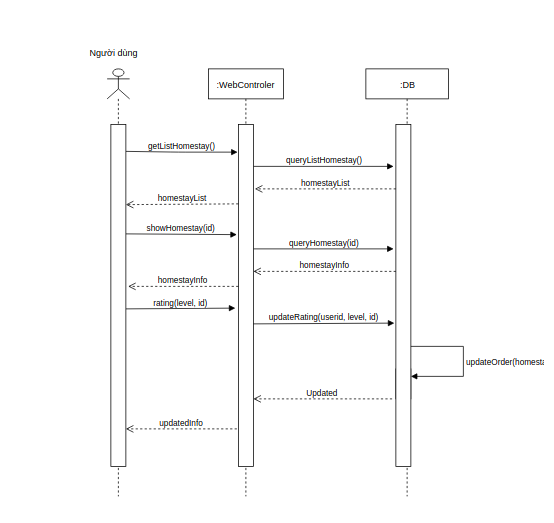
\includegraphics[width=13cm]{Image/tin-sequence-homstay-order.png}
        	\caption{Sequence Diagram cho usecase xếp hạng các homestay}
    \end{figure}
	\item \textbf{Usecase 3: Quản lý huy hiệu và xếp hạng các homestay.}
	\begin{center}
		\begin{longtable}{ | l |p{10cm}|}
			\hline
			\textbf{Tên usecase} & Quản lý huy hiệu và xếp hạng các homestay \\ \hline
			\textbf{Người tương tác} & Người dùng hệ thống \\ \hline   
			\textbf{Mô tả} &  Hệ thống tự động cập nhật huy hiệu và thứ hạng của nhà sau khi có 1 ratingmới của nhà xuất hiện. \\ \hline  
			\textbf{Người tạo:} \textit{Trần Ngọc Tín} & \textbf{Cập nhật lần cuối bởi:} \textit{Trần Ngọc Tín} \\ \hline
			\textbf{Ngày tạo:} \textit{22/03/2019} & \textbf{Lần cuối cập nhật:} \textit{30/03/2019} \\ \hline
			\textbf{Tiền điều kiện} &  Người dùng nào đó rating nhà. \\ \hline 
			\textbf{Hậu điều kiện} &  Thông tin về huy hiệu và thứ hạng của nhà đó được cập nhật \\ \hline 
			\textbf{Luồng cơ bản} & 
			\begin{enumerate}
		\item Người dùng rating nhà
		\item Hệ thống tính toán lại mức rating trung bình của nhà đó cũng như tổng số rating
		\item Hệ thống cập nhật lại huy hiệu cho nhà dựa theo mức rating trung bình và tổng số rating, chi tiết như sau:
		\begin{itemize}
		    \item Với nhà có tổng rating dưới 5: huy hiệu là "Nhà mới"
		    \item Với nhà đạt được tổng rating > 5 và <= 10: huy hiệu là "Nhà phổ biến"
		    \item Với nhà có tổng rating > 10, lúc này sẽ tính huy hiệu theo rating trung bình
		    \begin{itemize}
		        \item Với rating trung bình < 1: huy hiệu "Nhà quá tệ"
		        \item Với rating trung bình >= 1 và < 2: huy hiệu "Nhà tệ"
		        \item Với rating trung bình >= 2 và < 3: huy hiệu "Nhà tạm được"
		        \item Với rating trung bình >= 3 và < 4: huy hiệu "Nhà tốt"
		        \item Với rating trung bình >= 4 và <= 5: huy hiệu "Nhà tuyệt vời"
		    \end{itemize}
		\end{itemize}
		\item Hệ thống tính toán lại thứ tự ưu tiên của nhà theo mức rating trung bình mới, nhà nào có mức rating trung bình cao thì xếp hạng cao, nếu 2 nhà có mức rating trung bình bằng nhau thì dựa vào tổng số rating để xếp hạng, nhà nào có tổng rating cao hơn thì xếp hạng cao hơn
			\end{enumerate} \\ \hline
			\textbf{Luồng thay thế} & Không có \\ \hline
			\textbf{Ngoại lệ}  & Không có \\
			\hline
		\end{longtable}
	\end{center}
\end{enumerate}
\subsection{Module 3: Bình luận và rating cho nhà}
\begin{figure}[!h]
	\centering
	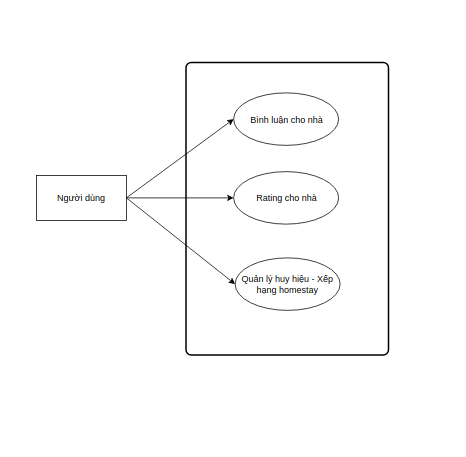
\includegraphics[width=10cm]{Image/tin-usecase.png}
	\caption{Lược đồ use case của Module 3: Bình luận và rating cho nhà}
\end{figure}
\subsubsection{User Story}
\textit{Diamond Stay} là một hệ thống trung gian giữa người cần thuê nhà và người cho thuê nhà. Hệ thống sẽ thu phí hoa hồng mỗi khi có lượt giao dịch thành công giữa chủ nhà và người cho thuê. Chủ nhà muốn thêm chỗ ở mới cần cho thuê thì cần gửi yêu cầu thêm chỗ ở mới lên hệ thống. Để thông tin về chỗ ở mới này xuất hiện trên trang web chính của \textit{Diamond Stay} để khách thuê nhà có thể thấy và đặt phòng thì tin đăng này cần phải được duyệt trước để đảm bảo tin đăng là hợp lệ, không phải là spam hay tin giả do một số đối tượng cố tình phá hoại hệ thống gửi lên. Những tin đăng loại này sẽ gây loãng hệ thống và gây khó khăn cho người dùng. Việc duyệt tin sẽ được những quản lí của hệ thống thực hiện. Hệ thống sẽ có một số tiêu chí để xác định tin đăng là hợp lệ hay không. Dựa vào đó quản lí có thể dựa vào để có thể quyết định trạng thái kế tiếp của 1 tin đăng. Các trạng thái này có thể là:
\begin{itemize}
	\item \textit{Thành công}: Tin đăng hợp lệ và được hiển thị lên trang web của Diamond Stay để khách thuê có thể nhìn thấy và đặt phòng 
	\item \textit{Bị từ chối}: Tin đăng không hợp lệ.
	\item \textit{Yêu cầu chỉnh sửa}: Tin đăng cần sửa đổi, bổ sung một số thông tin để hợp lệ. Chủ nhà sau khi sửa đổi và bổ sung có thể resubmit lại tin này.
\end{itemize}
Khi quản lí duyệt một tin là \textit{Bị từ chối} thì quản lí cần cung cấp lí do tin đăng bị từ chối, còn nếu tin đăng bị đánh giá là \textit{Yêu cầu chỉnh sửa} thì quản lí cần cung cấp chi tiết những nội dung nào cần chỉnh sửa, những nội dung nào chưa hợp lệ.
\subsubsection{Các usecase chi tiết}
\begin{figure}[!h]
	\centering
	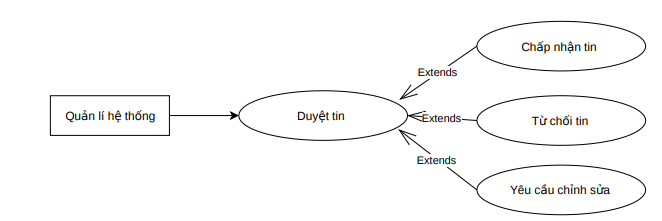
\includegraphics[width=12cm]{Image/module1.png}
	\vspace{0.5cm}
	\caption{Lược đồ use case của Module 1: Duyệt tin đăng yêu cầu thêm chỗ ở mới từ chủ nhà}
\end{figure}
\subsubsubsection{Use Case 1: Duyệt tin.}
\begin{figure}[!h]
	\centering
	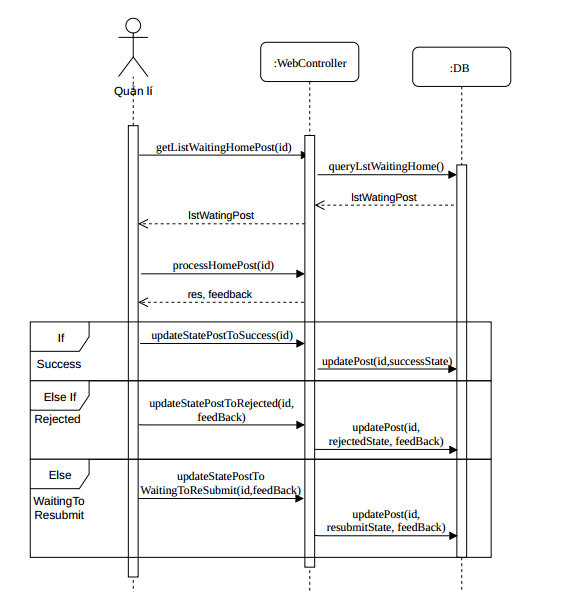
\includegraphics[width=13cm]{Image/duyetTinSequence.png}
	\caption{Sequence Diagram cho usecase Duyệt tin}
\end{figure}
\begin{center}
	\begin{longtable}{ | l |p{10cm}|}
		\hline
		\textbf{Tên usecase} & Duyệt tin \\ \hline
		\textbf{Người tương tác} & Quản lí hệ thống \\ \hline   
		\textbf{Mô tả} &  Cho phép người quản lí của hệ thống có thể duyệt qua các yêu cầu thêm nhà mới từ các chủ nhà. Việc duyệt tin để đảm bảo chất lượng của các bài đăng trên trang web của hệ thống.\\ \hline  
		\textbf{Người tạo:} \textit{Đinh Minh Tân} & \textbf{Cập nhật lần cuối bởi:} \textit{Đinh Minh Tân} \\ \hline
		\textbf{Ngày tạo:} \textit{22/03/2019} & \textbf{Lần cuối cập nhật:} \textit{30/03/2019} \\ \hline
		\textbf{Tiền điều kiện} &  Người dùng đã đăng nhập vào hệ thống bằng quyền của người quản lí, người dùng đang ở màn hình index của trang web. \\ \hline 
		\textbf{Hậu điều kiện} &  Quản lí quay về màn hình quản lí các tin chưa duyệt. \\ \hline 
		\textbf{Luồng cơ bản} & 
		\begin{enumerate}
			\item Quản lí nhấn tab Quản lí tin đăng.
			\item Hệ thống hiển thị 2 option cho quản lí bao gồm: Tin chưa duyệt, Tin đã duyệt.
			\item Quản lí chọn Tin chưa duyệt.
			\item Hệ thống hiển thị danh sách các tin chưa được duyệt, đang đợi duyệt.
			\item Người quản lí chọn một tin bất kì mà mình sẽ duyệt trong danh sách tin hiện ra.
			\item Hệ thống hiển thị tất cả thông tin của homestay cần được duyệt, trong đó có 3 option để duyệt: Chấp nhận, Từ chối và Yêu cầu chỉnh sửa.
			\item Quản lí sau khi duyệt tất cả các thông tin đầy đủ và hợp lệ, chọn option Chấp nhận và nhấn Button OK để xác nhận quyết định.
			\item Hệ thống hiện ra thông báo đã xác nhận thành công và tin đăng về homestay đã được đăng thành công lên trang web để khách thuê có thể thấy và đặt.
			\item Hệ thống quay về màn hình quản lí các tin chưa duyệt để quản lí có thể duyệt tin khác (nếu cần).
		\end{enumerate} \\ \hline 
		\textbf{Luồng thay thế} & 
		\begin{itemize} 
			\item \textit{Luồng thay thế 1}
			\begin{enumerate}
				\item Tại bước 4, hệ thống không tìm được tin nào chưa được duyệt thì sẽ in ra thông báo "Không có tin đăng nào cần duyệt" kết thúc chức năng này tại đây.
			\end{enumerate}
			
			\item \textit{Luồng thay thế 2}
			\begin{enumerate}
				\item Tại bước 6, quản lí chọn option Từ chối.
				\item Hệ thống hiện thị một form để quản lí điền lí do tin đăng bị từ chối. Sau khi hoàn thành xong form, quản lí nhấn OK.
				\item Hệ thống xác nhận tin đã bị từ chối và gửi kết quả về cho chủ nhà 
				\item Tiếp tục tại bước 9 của luồng cơ bản.
			\end{enumerate}
			
			\item \textit{Luồng thay thế 3}
			\begin{enumerate}
				\item Tại bước 6, quản lí chọn option Yêu cầu sửa đổi.
				\item Hệ thống hiện thị một form để quản lí điền những yêu cầu mà chủ nhà cần sửa đổi hoặc bổ sung thêm. Sau khi hoàn thành xong form, quản lí nhấn OK.
				\item Hệ thống đánh dấu chuyển tin sang dạng đợi và chuyển vào mục tin cần sửa đổi và resubmit lại bên phía chủ nhà.
				\item Tiếp tục tại bước 9 của luồng cơ bản.
			\end{enumerate}
		\end{itemize} \\ \hline 
		\textbf{Ngoại lệ}  & Không có \\
		\hline
	\end{longtable}
\end{center}
\subsubsection{Quản lý huy hiệu, xếp hạng các homestay}
\subsubsubsection{User Story}
\textit Từ kết quả rating,{Diamond Stay} sẽ quản lí huy hiệu và xếp hạng các homestay. Dựa trên cơ sở này, người dùng có thể dễ dàng biết được mức độ chuyên nghiệp cũng như chất lượng thực sự của homestay

\subsubsubsection{Mô tả các use case}
\begin{enumerate}[label=\textbf{(\alph*)}]
    \begin{figure}[!h]
        	\centering
        	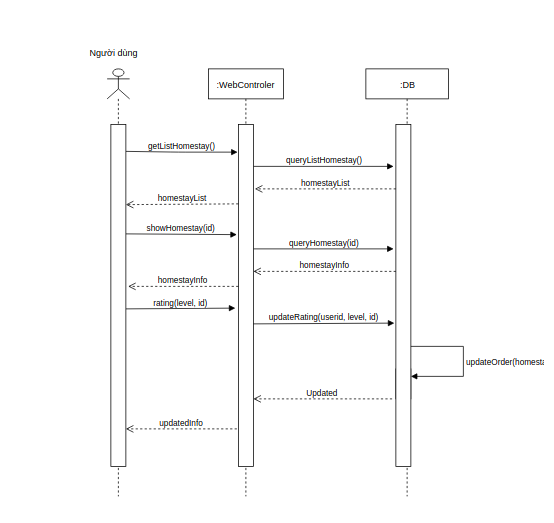
\includegraphics[width=13cm]{Image/tin-sequence-homstay-order.png}
        	\caption{Sequence Diagram cho usecase xếp hạng các homestay}
    \end{figure}
	\item \textbf{Usecase 3: Quản lý huy hiệu và xếp hạng các homestay.}
	\begin{center}
		\begin{longtable}{ | l |p{10cm}|}
			\hline
			\textbf{Tên usecase} & Quản lý huy hiệu và xếp hạng các homestay \\ \hline
			\textbf{Người tương tác} & Người dùng hệ thống \\ \hline   
			\textbf{Mô tả} &  Hệ thống tự động cập nhật huy hiệu và thứ hạng của nhà sau khi có 1 ratingmới của nhà xuất hiện. \\ \hline  
			\textbf{Người tạo:} \textit{Trần Ngọc Tín} & \textbf{Cập nhật lần cuối bởi:} \textit{Trần Ngọc Tín} \\ \hline
			\textbf{Ngày tạo:} \textit{22/03/2019} & \textbf{Lần cuối cập nhật:} \textit{30/03/2019} \\ \hline
			\textbf{Tiền điều kiện} &  Người dùng nào đó rating nhà. \\ \hline 
			\textbf{Hậu điều kiện} &  Thông tin về huy hiệu và thứ hạng của nhà đó được cập nhật \\ \hline 
			\textbf{Luồng cơ bản} & 
			\begin{enumerate}
		\item Người dùng rating nhà
		\item Hệ thống tính toán lại mức rating trung bình của nhà đó cũng như tổng số rating
		\item Hệ thống cập nhật lại huy hiệu cho nhà dựa theo mức rating trung bình và tổng số rating, chi tiết như sau:
		\begin{itemize}
		    \item Với nhà có tổng rating dưới 5: huy hiệu là "Nhà mới"
		    \item Với nhà đạt được tổng rating > 5 và <= 10: huy hiệu là "Nhà phổ biến"
		    \item Với nhà có tổng rating > 10, lúc này sẽ tính huy hiệu theo rating trung bình
		    \begin{itemize}
		        \item Với rating trung bình < 1: huy hiệu "Nhà quá tệ"
		        \item Với rating trung bình >= 1 và < 2: huy hiệu "Nhà tệ"
		        \item Với rating trung bình >= 2 và < 3: huy hiệu "Nhà tạm được"
		        \item Với rating trung bình >= 3 và < 4: huy hiệu "Nhà tốt"
		        \item Với rating trung bình >= 4 và <= 5: huy hiệu "Nhà tuyệt vời"
		    \end{itemize}
		\end{itemize}
		\item Hệ thống tính toán lại thứ tự ưu tiên của nhà theo mức rating trung bình mới, nhà nào có mức rating trung bình cao thì xếp hạng cao, nếu 2 nhà có mức rating trung bình bằng nhau thì dựa vào tổng số rating để xếp hạng, nhà nào có tổng rating cao hơn thì xếp hạng cao hơn
			\end{enumerate} \\ \hline
			\textbf{Luồng thay thế} & Không có \\ \hline
			\textbf{Ngoại lệ}  & Không có \\
			\hline
		\end{longtable}
	\end{center}
\end{enumerate}
\subsection{Module 3: Bình luận và rating cho nhà}
\begin{figure}[!h]
	\centering
	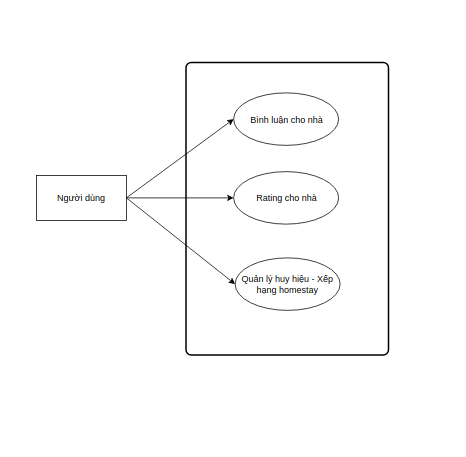
\includegraphics[width=10cm]{Image/tin-usecase.png}
	\caption{Lược đồ use case của Module 3: Bình luận và rating cho nhà}
\end{figure}
\subsubsection{User Story}
\textit{Diamond Stay} là một hệ thống trung gian giữa người cần thuê nhà và người cho thuê nhà. Hệ thống sẽ thu phí hoa hồng mỗi khi có lượt giao dịch thành công giữa chủ nhà và người cho thuê. Chủ nhà muốn thêm chỗ ở mới cần cho thuê thì cần gửi yêu cầu thêm chỗ ở mới lên hệ thống. Để thông tin về chỗ ở mới này xuất hiện trên trang web chính của \textit{Diamond Stay} để khách thuê nhà có thể thấy và đặt phòng thì tin đăng này cần phải được duyệt trước để đảm bảo tin đăng là hợp lệ, không phải là spam hay tin giả do một số đối tượng cố tình phá hoại hệ thống gửi lên. Những tin đăng loại này sẽ gây loãng hệ thống và gây khó khăn cho người dùng. Việc duyệt tin sẽ được những quản lí của hệ thống thực hiện. Hệ thống sẽ có một số tiêu chí để xác định tin đăng là hợp lệ hay không. Dựa vào đó quản lí có thể dựa vào để có thể quyết định trạng thái kế tiếp của 1 tin đăng. Các trạng thái này có thể là:
\begin{itemize}
	\item \textit{Thành công}: Tin đăng hợp lệ và được hiển thị lên trang web của Diamond Stay để khách thuê có thể nhìn thấy và đặt phòng 
	\item \textit{Bị từ chối}: Tin đăng không hợp lệ.
	\item \textit{Yêu cầu chỉnh sửa}: Tin đăng cần sửa đổi, bổ sung một số thông tin để hợp lệ. Chủ nhà sau khi sửa đổi và bổ sung có thể resubmit lại tin này.
\end{itemize}
Khi quản lí duyệt một tin là \textit{Bị từ chối} thì quản lí cần cung cấp lí do tin đăng bị từ chối, còn nếu tin đăng bị đánh giá là \textit{Yêu cầu chỉnh sửa} thì quản lí cần cung cấp chi tiết những nội dung nào cần chỉnh sửa, những nội dung nào chưa hợp lệ.
\subsubsection{Các usecase chi tiết}
\begin{figure}[!h]
	\centering
	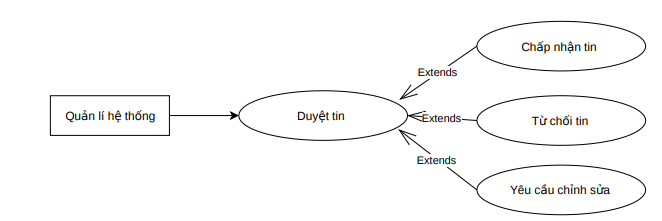
\includegraphics[width=12cm]{Image/module1.png}
	\vspace{0.5cm}
	\caption{Lược đồ use case của Module 1: Duyệt tin đăng yêu cầu thêm chỗ ở mới từ chủ nhà}
\end{figure}
\subsubsubsection{Use Case 1: Duyệt tin.}
\begin{figure}[!h]
	\centering
	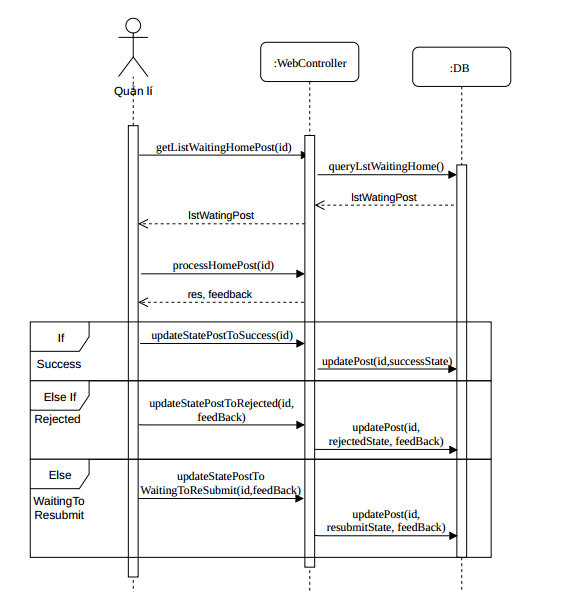
\includegraphics[width=13cm]{Image/duyetTinSequence.png}
	\caption{Sequence Diagram cho usecase Duyệt tin}
\end{figure}
\begin{center}
	\begin{longtable}{ | l |p{10cm}|}
		\hline
		\textbf{Tên usecase} & Duyệt tin \\ \hline
		\textbf{Người tương tác} & Quản lí hệ thống \\ \hline   
		\textbf{Mô tả} &  Cho phép người quản lí của hệ thống có thể duyệt qua các yêu cầu thêm nhà mới từ các chủ nhà. Việc duyệt tin để đảm bảo chất lượng của các bài đăng trên trang web của hệ thống.\\ \hline  
		\textbf{Người tạo:} \textit{Đinh Minh Tân} & \textbf{Cập nhật lần cuối bởi:} \textit{Đinh Minh Tân} \\ \hline
		\textbf{Ngày tạo:} \textit{22/03/2019} & \textbf{Lần cuối cập nhật:} \textit{30/03/2019} \\ \hline
		\textbf{Tiền điều kiện} &  Người dùng đã đăng nhập vào hệ thống bằng quyền của người quản lí, người dùng đang ở màn hình index của trang web. \\ \hline 
		\textbf{Hậu điều kiện} &  Quản lí quay về màn hình quản lí các tin chưa duyệt. \\ \hline 
		\textbf{Luồng cơ bản} & 
		\begin{enumerate}
			\item Quản lí nhấn tab Quản lí tin đăng.
			\item Hệ thống hiển thị 2 option cho quản lí bao gồm: Tin chưa duyệt, Tin đã duyệt.
			\item Quản lí chọn Tin chưa duyệt.
			\item Hệ thống hiển thị danh sách các tin chưa được duyệt, đang đợi duyệt.
			\item Người quản lí chọn một tin bất kì mà mình sẽ duyệt trong danh sách tin hiện ra.
			\item Hệ thống hiển thị tất cả thông tin của homestay cần được duyệt, trong đó có 3 option để duyệt: Chấp nhận, Từ chối và Yêu cầu chỉnh sửa.
			\item Quản lí sau khi duyệt tất cả các thông tin đầy đủ và hợp lệ, chọn option Chấp nhận và nhấn Button OK để xác nhận quyết định.
			\item Hệ thống hiện ra thông báo đã xác nhận thành công và tin đăng về homestay đã được đăng thành công lên trang web để khách thuê có thể thấy và đặt.
			\item Hệ thống quay về màn hình quản lí các tin chưa duyệt để quản lí có thể duyệt tin khác (nếu cần).
		\end{enumerate} \\ \hline 
		\textbf{Luồng thay thế} & 
		\begin{itemize} 
			\item \textit{Luồng thay thế 1}
			\begin{enumerate}
				\item Tại bước 4, hệ thống không tìm được tin nào chưa được duyệt thì sẽ in ra thông báo "Không có tin đăng nào cần duyệt" kết thúc chức năng này tại đây.
			\end{enumerate}
			
			\item \textit{Luồng thay thế 2}
			\begin{enumerate}
				\item Tại bước 6, quản lí chọn option Từ chối.
				\item Hệ thống hiện thị một form để quản lí điền lí do tin đăng bị từ chối. Sau khi hoàn thành xong form, quản lí nhấn OK.
				\item Hệ thống xác nhận tin đã bị từ chối và gửi kết quả về cho chủ nhà 
				\item Tiếp tục tại bước 9 của luồng cơ bản.
			\end{enumerate}
			
			\item \textit{Luồng thay thế 3}
			\begin{enumerate}
				\item Tại bước 6, quản lí chọn option Yêu cầu sửa đổi.
				\item Hệ thống hiện thị một form để quản lí điền những yêu cầu mà chủ nhà cần sửa đổi hoặc bổ sung thêm. Sau khi hoàn thành xong form, quản lí nhấn OK.
				\item Hệ thống đánh dấu chuyển tin sang dạng đợi và chuyển vào mục tin cần sửa đổi và resubmit lại bên phía chủ nhà.
				\item Tiếp tục tại bước 9 của luồng cơ bản.
			\end{enumerate}
		\end{itemize} \\ \hline 
		\textbf{Ngoại lệ}  & Không có \\
		\hline
	\end{longtable}
\end{center}
\subsubsection{Quản lý huy hiệu, xếp hạng các homestay}
\subsubsubsection{User Story}
\textit Từ kết quả rating,{Diamond Stay} sẽ quản lí huy hiệu và xếp hạng các homestay. Dựa trên cơ sở này, người dùng có thể dễ dàng biết được mức độ chuyên nghiệp cũng như chất lượng thực sự của homestay

\subsubsubsection{Mô tả các use case}
\begin{enumerate}[label=\textbf{(\alph*)}]
    \begin{figure}[!h]
        	\centering
        	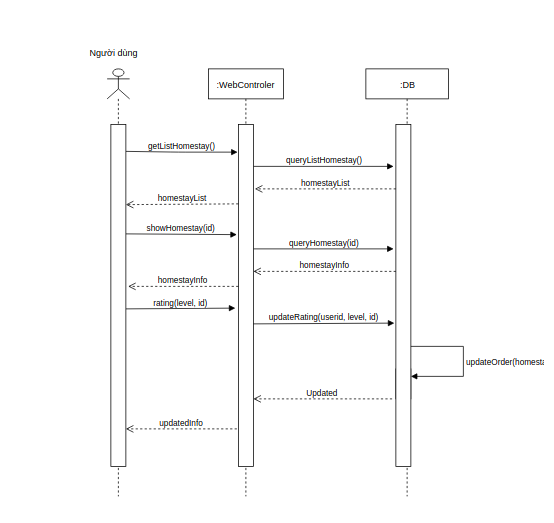
\includegraphics[width=13cm]{Image/tin-sequence-homstay-order.png}
        	\caption{Sequence Diagram cho usecase xếp hạng các homestay}
    \end{figure}
	\item \textbf{Usecase 3: Quản lý huy hiệu và xếp hạng các homestay.}
	\begin{center}
		\begin{longtable}{ | l |p{10cm}|}
			\hline
			\textbf{Tên usecase} & Quản lý huy hiệu và xếp hạng các homestay \\ \hline
			\textbf{Người tương tác} & Người dùng hệ thống \\ \hline   
			\textbf{Mô tả} &  Hệ thống tự động cập nhật huy hiệu và thứ hạng của nhà sau khi có 1 ratingmới của nhà xuất hiện. \\ \hline  
			\textbf{Người tạo:} \textit{Trần Ngọc Tín} & \textbf{Cập nhật lần cuối bởi:} \textit{Trần Ngọc Tín} \\ \hline
			\textbf{Ngày tạo:} \textit{22/03/2019} & \textbf{Lần cuối cập nhật:} \textit{30/03/2019} \\ \hline
			\textbf{Tiền điều kiện} &  Người dùng nào đó rating nhà. \\ \hline 
			\textbf{Hậu điều kiện} &  Thông tin về huy hiệu và thứ hạng của nhà đó được cập nhật \\ \hline 
			\textbf{Luồng cơ bản} & 
			\begin{enumerate}
		\item Người dùng rating nhà
		\item Hệ thống tính toán lại mức rating trung bình của nhà đó cũng như tổng số rating
		\item Hệ thống cập nhật lại huy hiệu cho nhà dựa theo mức rating trung bình và tổng số rating, chi tiết như sau:
		\begin{itemize}
		    \item Với nhà có tổng rating dưới 5: huy hiệu là "Nhà mới"
		    \item Với nhà đạt được tổng rating > 5 và <= 10: huy hiệu là "Nhà phổ biến"
		    \item Với nhà có tổng rating > 10, lúc này sẽ tính huy hiệu theo rating trung bình
		    \begin{itemize}
		        \item Với rating trung bình < 1: huy hiệu "Nhà quá tệ"
		        \item Với rating trung bình >= 1 và < 2: huy hiệu "Nhà tệ"
		        \item Với rating trung bình >= 2 và < 3: huy hiệu "Nhà tạm được"
		        \item Với rating trung bình >= 3 và < 4: huy hiệu "Nhà tốt"
		        \item Với rating trung bình >= 4 và <= 5: huy hiệu "Nhà tuyệt vời"
		    \end{itemize}
		\end{itemize}
		\item Hệ thống tính toán lại thứ tự ưu tiên của nhà theo mức rating trung bình mới, nhà nào có mức rating trung bình cao thì xếp hạng cao, nếu 2 nhà có mức rating trung bình bằng nhau thì dựa vào tổng số rating để xếp hạng, nhà nào có tổng rating cao hơn thì xếp hạng cao hơn
			\end{enumerate} \\ \hline
			\textbf{Luồng thay thế} & Không có \\ \hline
			\textbf{Ngoại lệ}  & Không có \\
			\hline
		\end{longtable}
	\end{center}
\end{enumerate}
\subsection{Module 3: Bình luận và rating cho nhà}
\begin{figure}[!h]
	\centering
	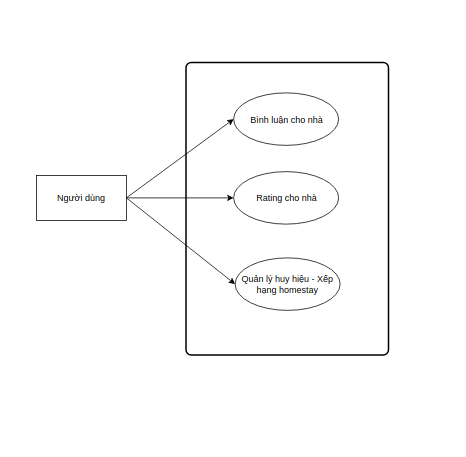
\includegraphics[width=10cm]{Image/tin-usecase.png}
	\caption{Lược đồ use case của Module 3: Bình luận và rating cho nhà}
\end{figure}
\subsubsection{User Story}
\textit{Diamond Stay} là một hệ thống trung gian giữa người cần thuê nhà và người cho thuê nhà. Hệ thống sẽ thu phí hoa hồng mỗi khi có lượt giao dịch thành công giữa chủ nhà và người cho thuê. Chủ nhà muốn thêm chỗ ở mới cần cho thuê thì cần gửi yêu cầu thêm chỗ ở mới lên hệ thống. Để thông tin về chỗ ở mới này xuất hiện trên trang web chính của \textit{Diamond Stay} để khách thuê nhà có thể thấy và đặt phòng thì tin đăng này cần phải được duyệt trước để đảm bảo tin đăng là hợp lệ, không phải là spam hay tin giả do một số đối tượng cố tình phá hoại hệ thống gửi lên. Những tin đăng loại này sẽ gây loãng hệ thống và gây khó khăn cho người dùng. Việc duyệt tin sẽ được những quản lí của hệ thống thực hiện. Hệ thống sẽ có một số tiêu chí để xác định tin đăng là hợp lệ hay không. Dựa vào đó quản lí có thể dựa vào để có thể quyết định trạng thái kế tiếp của 1 tin đăng. Các trạng thái này có thể là:
\begin{itemize}
	\item \textit{Thành công}: Tin đăng hợp lệ và được hiển thị lên trang web của Diamond Stay để khách thuê có thể nhìn thấy và đặt phòng 
	\item \textit{Bị từ chối}: Tin đăng không hợp lệ.
	\item \textit{Yêu cầu chỉnh sửa}: Tin đăng cần sửa đổi, bổ sung một số thông tin để hợp lệ. Chủ nhà sau khi sửa đổi và bổ sung có thể resubmit lại tin này.
\end{itemize}
Khi quản lí duyệt một tin là \textit{Bị từ chối} thì quản lí cần cung cấp lí do tin đăng bị từ chối, còn nếu tin đăng bị đánh giá là \textit{Yêu cầu chỉnh sửa} thì quản lí cần cung cấp chi tiết những nội dung nào cần chỉnh sửa, những nội dung nào chưa hợp lệ.
\subsubsection{Các usecase chi tiết}
\begin{figure}[!h]
	\centering
	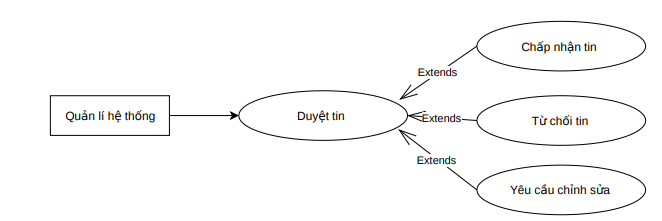
\includegraphics[width=12cm]{Image/module1.png}
	\vspace{0.5cm}
	\caption{Lược đồ use case của Module 1: Duyệt tin đăng yêu cầu thêm chỗ ở mới từ chủ nhà}
\end{figure}
\subsubsubsection{Use Case 1: Duyệt tin.}
\begin{figure}[!h]
	\centering
	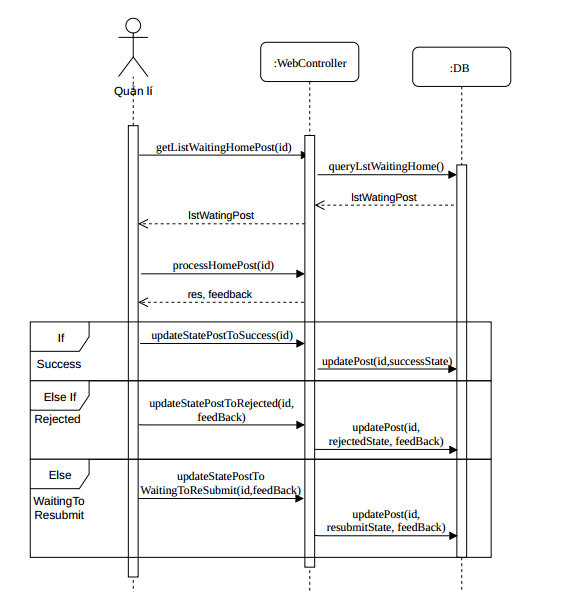
\includegraphics[width=13cm]{Image/duyetTinSequence.png}
	\caption{Sequence Diagram cho usecase Duyệt tin}
\end{figure}
\begin{center}
	\begin{longtable}{ | l |p{10cm}|}
		\hline
		\textbf{Tên usecase} & Duyệt tin \\ \hline
		\textbf{Người tương tác} & Quản lí hệ thống \\ \hline   
		\textbf{Mô tả} &  Cho phép người quản lí của hệ thống có thể duyệt qua các yêu cầu thêm nhà mới từ các chủ nhà. Việc duyệt tin để đảm bảo chất lượng của các bài đăng trên trang web của hệ thống.\\ \hline  
		\textbf{Người tạo:} \textit{Đinh Minh Tân} & \textbf{Cập nhật lần cuối bởi:} \textit{Đinh Minh Tân} \\ \hline
		\textbf{Ngày tạo:} \textit{22/03/2019} & \textbf{Lần cuối cập nhật:} \textit{30/03/2019} \\ \hline
		\textbf{Tiền điều kiện} &  Người dùng đã đăng nhập vào hệ thống bằng quyền của người quản lí, người dùng đang ở màn hình index của trang web. \\ \hline 
		\textbf{Hậu điều kiện} &  Quản lí quay về màn hình quản lí các tin chưa duyệt. \\ \hline 
		\textbf{Luồng cơ bản} & 
		\begin{enumerate}
			\item Quản lí nhấn tab Quản lí tin đăng.
			\item Hệ thống hiển thị 2 option cho quản lí bao gồm: Tin chưa duyệt, Tin đã duyệt.
			\item Quản lí chọn Tin chưa duyệt.
			\item Hệ thống hiển thị danh sách các tin chưa được duyệt, đang đợi duyệt.
			\item Người quản lí chọn một tin bất kì mà mình sẽ duyệt trong danh sách tin hiện ra.
			\item Hệ thống hiển thị tất cả thông tin của homestay cần được duyệt, trong đó có 3 option để duyệt: Chấp nhận, Từ chối và Yêu cầu chỉnh sửa.
			\item Quản lí sau khi duyệt tất cả các thông tin đầy đủ và hợp lệ, chọn option Chấp nhận và nhấn Button OK để xác nhận quyết định.
			\item Hệ thống hiện ra thông báo đã xác nhận thành công và tin đăng về homestay đã được đăng thành công lên trang web để khách thuê có thể thấy và đặt.
			\item Hệ thống quay về màn hình quản lí các tin chưa duyệt để quản lí có thể duyệt tin khác (nếu cần).
		\end{enumerate} \\ \hline 
		\textbf{Luồng thay thế} & 
		\begin{itemize} 
			\item \textit{Luồng thay thế 1}
			\begin{enumerate}
				\item Tại bước 4, hệ thống không tìm được tin nào chưa được duyệt thì sẽ in ra thông báo "Không có tin đăng nào cần duyệt" kết thúc chức năng này tại đây.
			\end{enumerate}
			
			\item \textit{Luồng thay thế 2}
			\begin{enumerate}
				\item Tại bước 6, quản lí chọn option Từ chối.
				\item Hệ thống hiện thị một form để quản lí điền lí do tin đăng bị từ chối. Sau khi hoàn thành xong form, quản lí nhấn OK.
				\item Hệ thống xác nhận tin đã bị từ chối và gửi kết quả về cho chủ nhà 
				\item Tiếp tục tại bước 9 của luồng cơ bản.
			\end{enumerate}
			
			\item \textit{Luồng thay thế 3}
			\begin{enumerate}
				\item Tại bước 6, quản lí chọn option Yêu cầu sửa đổi.
				\item Hệ thống hiện thị một form để quản lí điền những yêu cầu mà chủ nhà cần sửa đổi hoặc bổ sung thêm. Sau khi hoàn thành xong form, quản lí nhấn OK.
				\item Hệ thống đánh dấu chuyển tin sang dạng đợi và chuyển vào mục tin cần sửa đổi và resubmit lại bên phía chủ nhà.
				\item Tiếp tục tại bước 9 của luồng cơ bản.
			\end{enumerate}
		\end{itemize} \\ \hline 
		\textbf{Ngoại lệ}  & Không có \\
		\hline
	\end{longtable}
\end{center}
\subsubsection{Quản lý huy hiệu, xếp hạng các homestay}
\subsubsubsection{User Story}
\textit Từ kết quả rating,{Diamond Stay} sẽ quản lí huy hiệu và xếp hạng các homestay. Dựa trên cơ sở này, người dùng có thể dễ dàng biết được mức độ chuyên nghiệp cũng như chất lượng thực sự của homestay

\subsubsubsection{Mô tả các use case}
\begin{enumerate}[label=\textbf{(\alph*)}]
    \begin{figure}[!h]
        	\centering
        	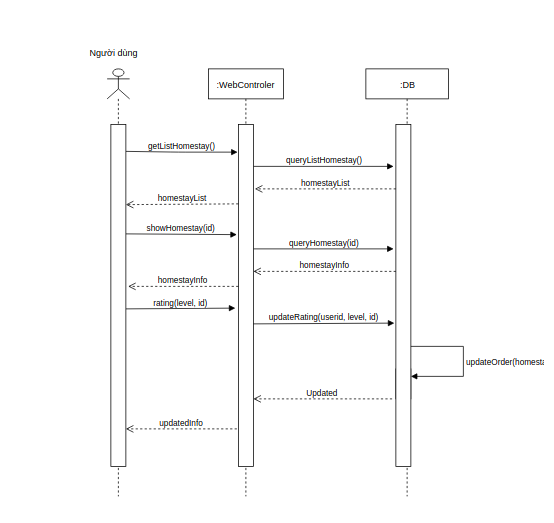
\includegraphics[width=13cm]{Image/tin-sequence-homstay-order.png}
        	\caption{Sequence Diagram cho usecase xếp hạng các homestay}
    \end{figure}
	\item \textbf{Usecase 3: Quản lý huy hiệu và xếp hạng các homestay.}
	\begin{center}
		\begin{longtable}{ | l |p{10cm}|}
			\hline
			\textbf{Tên usecase} & Quản lý huy hiệu và xếp hạng các homestay \\ \hline
			\textbf{Người tương tác} & Người dùng hệ thống \\ \hline   
			\textbf{Mô tả} &  Hệ thống tự động cập nhật huy hiệu và thứ hạng của nhà sau khi có 1 ratingmới của nhà xuất hiện. \\ \hline  
			\textbf{Người tạo:} \textit{Trần Ngọc Tín} & \textbf{Cập nhật lần cuối bởi:} \textit{Trần Ngọc Tín} \\ \hline
			\textbf{Ngày tạo:} \textit{22/03/2019} & \textbf{Lần cuối cập nhật:} \textit{30/03/2019} \\ \hline
			\textbf{Tiền điều kiện} &  Người dùng nào đó rating nhà. \\ \hline 
			\textbf{Hậu điều kiện} &  Thông tin về huy hiệu và thứ hạng của nhà đó được cập nhật \\ \hline 
			\textbf{Luồng cơ bản} & 
			\begin{enumerate}
		\item Người dùng rating nhà
		\item Hệ thống tính toán lại mức rating trung bình của nhà đó cũng như tổng số rating
		\item Hệ thống cập nhật lại huy hiệu cho nhà dựa theo mức rating trung bình và tổng số rating, chi tiết như sau:
		\begin{itemize}
		    \item Với nhà có tổng rating dưới 5: huy hiệu là "Nhà mới"
		    \item Với nhà đạt được tổng rating > 5 và <= 10: huy hiệu là "Nhà phổ biến"
		    \item Với nhà có tổng rating > 10, lúc này sẽ tính huy hiệu theo rating trung bình
		    \begin{itemize}
		        \item Với rating trung bình < 1: huy hiệu "Nhà quá tệ"
		        \item Với rating trung bình >= 1 và < 2: huy hiệu "Nhà tệ"
		        \item Với rating trung bình >= 2 và < 3: huy hiệu "Nhà tạm được"
		        \item Với rating trung bình >= 3 và < 4: huy hiệu "Nhà tốt"
		        \item Với rating trung bình >= 4 và <= 5: huy hiệu "Nhà tuyệt vời"
		    \end{itemize}
		\end{itemize}
		\item Hệ thống tính toán lại thứ tự ưu tiên của nhà theo mức rating trung bình mới, nhà nào có mức rating trung bình cao thì xếp hạng cao, nếu 2 nhà có mức rating trung bình bằng nhau thì dựa vào tổng số rating để xếp hạng, nhà nào có tổng rating cao hơn thì xếp hạng cao hơn
			\end{enumerate} \\ \hline
			\textbf{Luồng thay thế} & Không có \\ \hline
			\textbf{Ngoại lệ}  & Không có \\
			\hline
		\end{longtable}
	\end{center}
\end{enumerate}

%%%%%%% NON FUNCTIONAL %%%%%%%%%%
\section{Đặc tả các yêu cầu phi chức năng}
\subsection{Availability Requirements}
\begin{itemize}
	\item Hệ thống luôn sẵn sàng vào cuối tuần hoặc những ngày lễ .
\end{itemize}


\subsection{Security Requirements}
\begin{itemize}
	\item Người dùng không thể xem được các thông tin của người dùng khác trừ tên của họ.
\end{itemize}

\subsection{Usability Requirements}
\begin{itemize}
	\item Hệ thống nên dễ sử dụng, người dùng có thể hiểu và sử dụng thành thạo các chức năng của hệ thống trong vòng 2 giờ được hướng dẫn
	\item Hệ thống cần có ít nhất một tài liệu hướng dẫn cho các chức năng đăng tin, quản lý khuyến mãi. Các tài liệu này xuất hiện trong tab Helps. 
\end{itemize}

\subsection{Scalabitlity Requirements}
\begin{itemize}
	\item Hệ thống cần đảm bảo cho ít nhất 1000 người truy cập cùng một lúc mà không bị quá tải.
\end{itemize}

\subsection{Performance Requirements}
\begin{itemize}
	\item Thời gian để phản hồi của đa số chức năng của hệ thống không quá 5 giây.
\end{itemize}

%%%%%%% Architechture Design %%%%
\newpage 
\section{Kiến trúc hệ thống}
\begin{figure}[H]
	\centering
	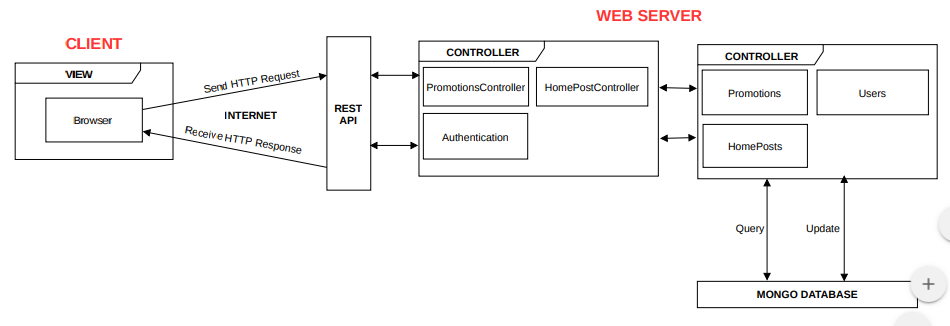
\includegraphics[width=14cm]{Image/ar.png}
	\vspace{0.5cm}
	\caption{Kiến trúc hệ thống}
\end{figure}

Mẫu thiết kế được dùng cho hệ thống chia sẻ nhà DiamondStay là MCV (Model-Controller-View) dành cho web. Mô hình này khá phổ biến cho các ứng dụng web.

%%%%%%% Class Diagram %%%%%%%%%%%
\newpage 
\section{Thiết kế lược đồ class}
\begin{figure}[H]
	\centering
	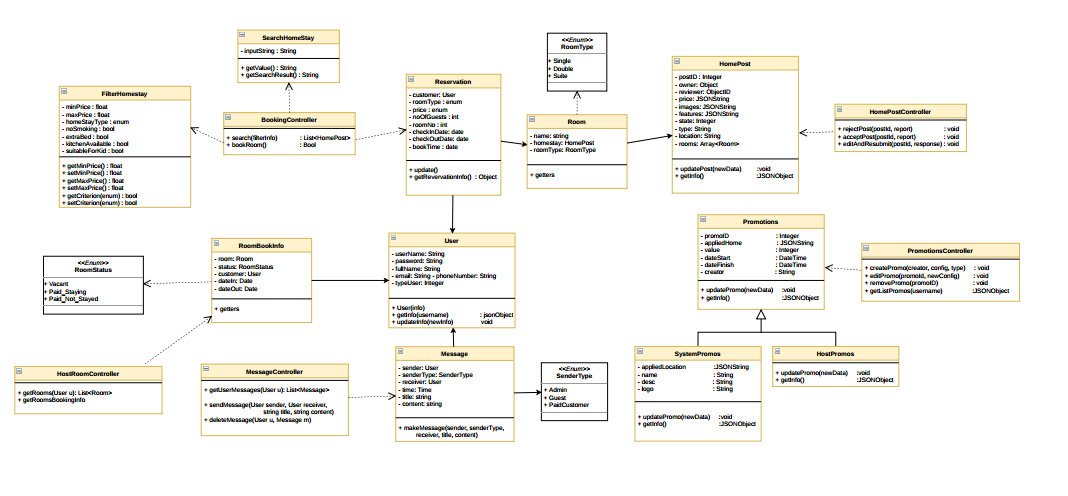
\includegraphics[width=14cm]{Image/777.png}
	\vspace{0.5cm}
	\caption{Lược đồ class của Diamond Stay}
\end{figure}
\subsection{Class Users}
\begin{figure}[H]
	\centering
	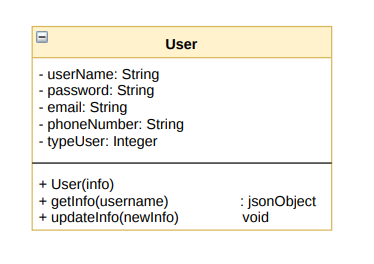
\includegraphics[width=7cm]{Image/444.png}
	\vspace{0.5cm}
	\caption{Lược đồ class Users}
\end{figure}
\subsection{Lược đồ class cho module Quản lí khuyến mại}
\begin{figure}[H]
	\centering
	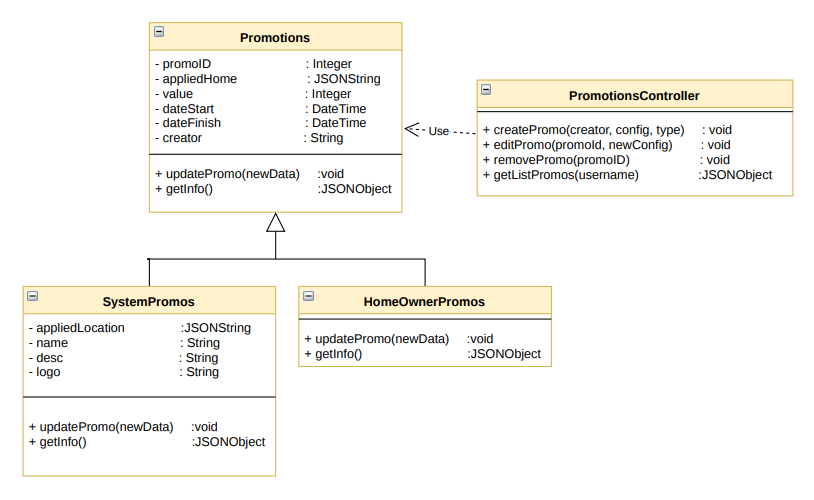
\includegraphics[width=10cm]{Image/555.png}
	\vspace{0.5cm}
	\caption{Lược đồ class cho module Quản lí khuyến mại}
\end{figure}
\subsection{Lược đồ class cho module Duyệt tin}
\begin{figure}[H]
	\centering
	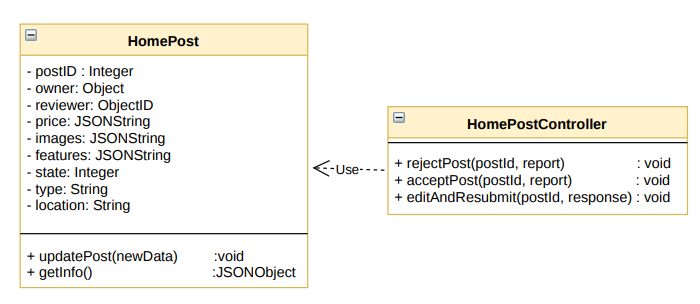
\includegraphics[width=10cm]{Image/333.png}
	\vspace{0.5cm}
	\caption{Lược đồ class cho module Duyệt tin}
\end{figure}

%%%%%%% Detailed Usecase %%%%%%%%
\section{Usecase chi tiết mức thiết kế}
\subsection{Lấy danh sách khuyến mại}
\begin{figure}[H]
	\centering
	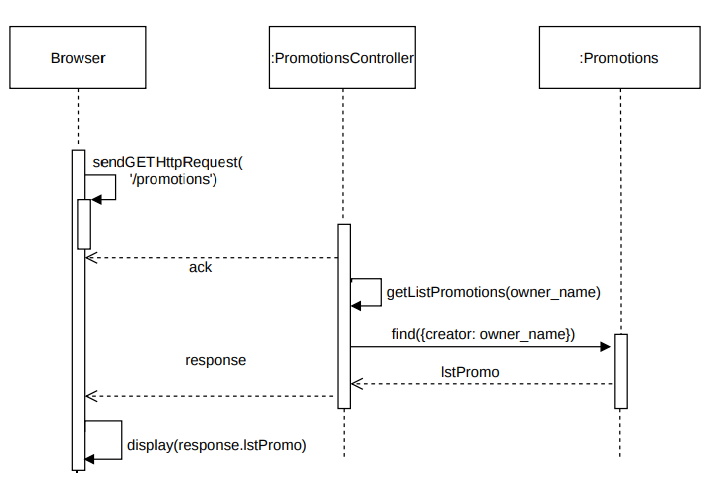
\includegraphics[width=12cm]{Image/223.png}
	\vspace{0.5cm}
	\caption{Sequence Diagram mức thiết kế cho usecase: Lấy danh sách khuyến mại}
\end{figure}
\subsection{Xóa khuyến mại}
\begin{figure}[H]
	\centering
	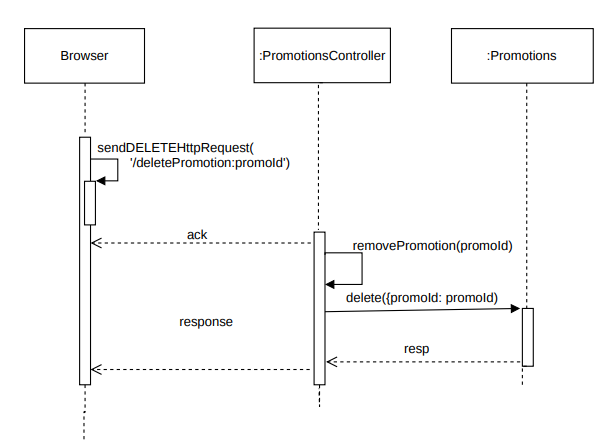
\includegraphics[width=12cm]{Image/rmPro.png}
	\vspace{0.5cm}
	\caption{Sequence Diagram mức thiết kế cho usecase: Xóa khuyến mại}
\end{figure}
\subsection{Tạo khuyến mại}
\begin{figure}[H]
	\centering
	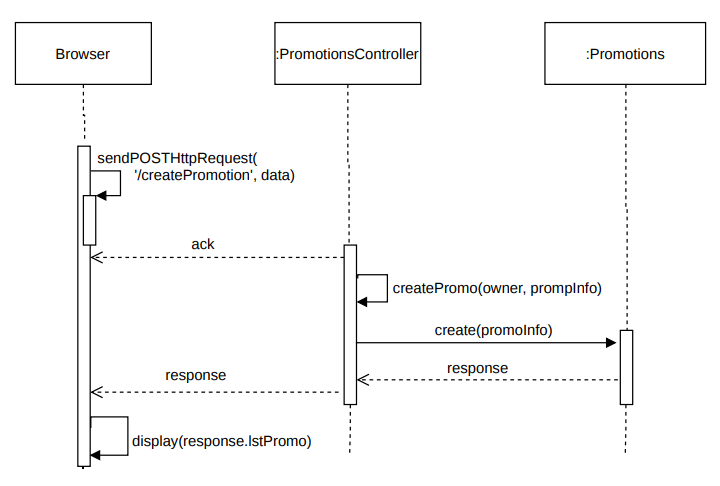
\includegraphics[width=12cm]{Image/cr2.png}
	\vspace{0.5cm}
	\caption{Sequence Diagram mức thiết kế cho usecase: Tạo khuyến mại}
\end{figure}
\subsection{Chỉnh sửa khuyến mại}
\begin{figure}[H]
	\centering
	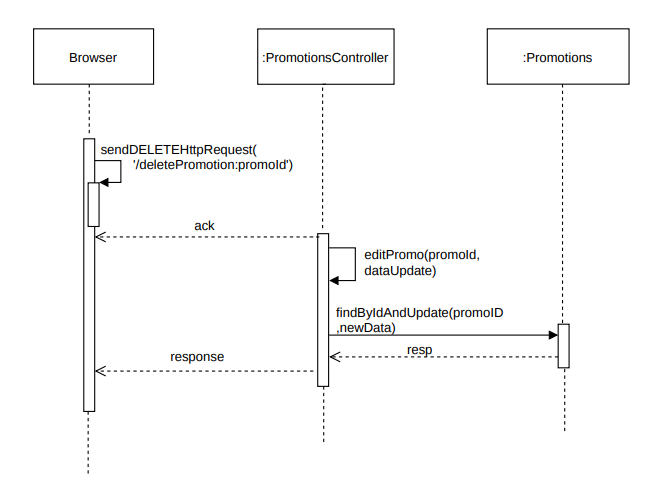
\includegraphics[width=12cm]{Image/cs.png}
	\vspace{0.5cm}
	\caption{Sequence Diagram mức thiết kế cho usecase: Chỉnh sửa khuyến mại}
\end{figure}

%%%%%%% UI %%%%%%%%%%%%%%%%%%%%%%
\subsection{Module 6: Theo dõi tình trạng đặt phòng}
\begin{figure}[H]
	\centering
	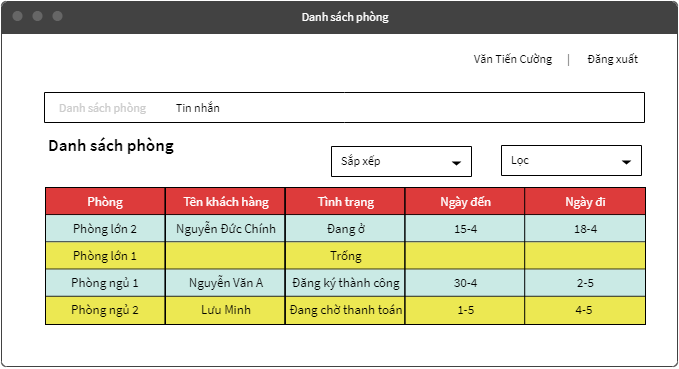
\includegraphics[width=10cm]{parts/Cuong/images/danh-sach-phong.png}
	\vspace{0.5cm}
	\caption{Giao diện: Xem danh sách phòng}
\end{figure}

\subsection{Module 8: Tin nhắn cho chủ nhà}
\subsubsection{Giao diện xem danh sách tin nhắn}
\begin{figure}[H]
	\centering
	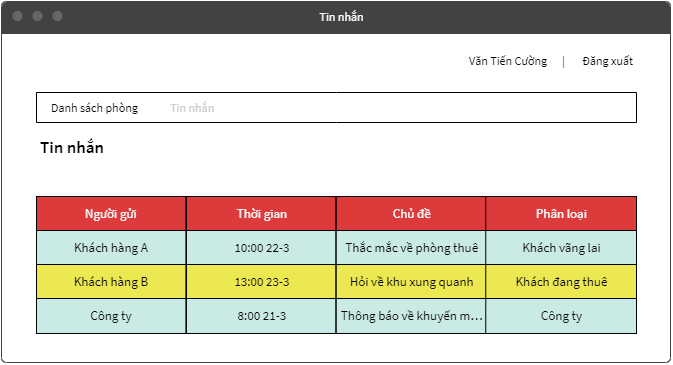
\includegraphics[width=10cm]{parts/Cuong/images/ds-tin-nhan.png}
	\vspace{0.5cm}
	\caption{Giao diện: Xem danh sách tin nhắn}
\end{figure}

\newpage 
\subsubsection{Giao diện xem chi tiết tin nhắn}
\begin{figure}[H]
	\centering
	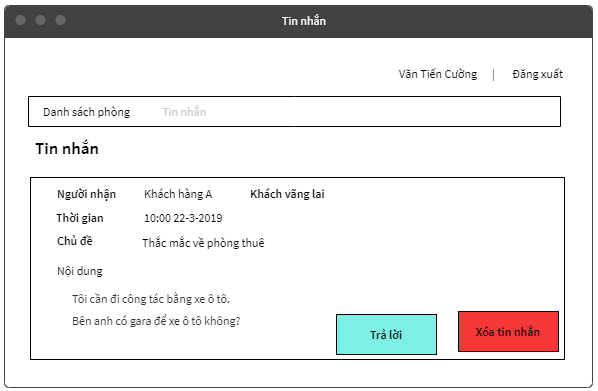
\includegraphics[width=10cm]{parts/Cuong/images/chi-tiet-tin-nhan.png}
	\vspace{0.5cm}
	\caption{Giao diện: Xem chi tiết tin nhắn}
\end{figure}
\subsubsection{Giao diện trả lời tin nhắn}
\begin{figure}[H]
	\centering
	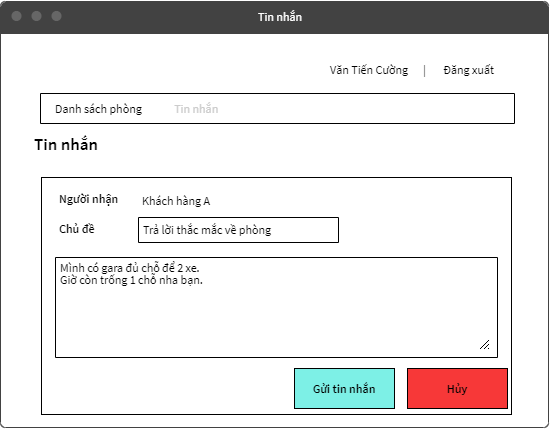
\includegraphics[width=8cm]{parts/Cuong/images/tra-loi-tin-nhan.png}
	\vspace{0.5cm}
	\caption{Giao diện: Trả lời tin nhắn}
\end{figure}

%%%%%%% UI %%%%%%%%%%%%%%%%%%%%%%
\newpage 
\section{Hiện thực hệ thống}
\underline{\textbf{Source code:}} \url{https://github.com/di-mi-ta/DiamondStay} \textit{(On going)}

\end{document}

